\documentclass[french]{article}
\usepackage[T1]{fontenc}
\usepackage[utf8]{inputenc}
\usepackage{lipsum}
\usepackage{lmodern}
\usepackage{geometry}
\usepackage{babel}
\usepackage{graphicx}
\usepackage{lastpage}
\usepackage{ragged2e}
\usepackage{enumitem}
\usepackage{multicol}

\geometry{
 	a4paper,
 	total={210mm,297mm},
 	left=20mm,
 	right=20mm,
 	top=20mm,
 	bottom=20mm,
}

\usepackage{fancyhdr}
\pagestyle{fancy}
\setlist[enumerate,1]{leftmargin=2cm}

\lhead{Damien Rochat <damien.rochat@heig-vd.ch>\\https://github.com/damienrochat/Teaching-HEIGVD-RES}
\chead{}
\rhead{08.03.2016}
\lfoot{HEIG-VD - RES}
\cfoot{}
\rfoot{page \thepage{} sur \pageref{LastPage}}
\renewcommand{\headrulewidth}{0.4pt}
\renewcommand{\footrulewidth}{0.4pt}

\begin{document}
	\centering
	\large{\textbf{RES : exemple 01 "BufferedIOBenchmark"}}
	
	\justify
	
	\section{Présentation}
		\noindent Ce programme à pour objectif de permettre de visualiser les différences en terme de durée d'écriture et de lecture lors de l'utilisation ou non des buffers d'entrées/sorties. \\
		
		\noindent Les tests ont été effectués sur un ordinateur Macbook Pro 2013, Intel Core i7 2.3 GHz. \\
		
	\section{Résultats}
		\centering
		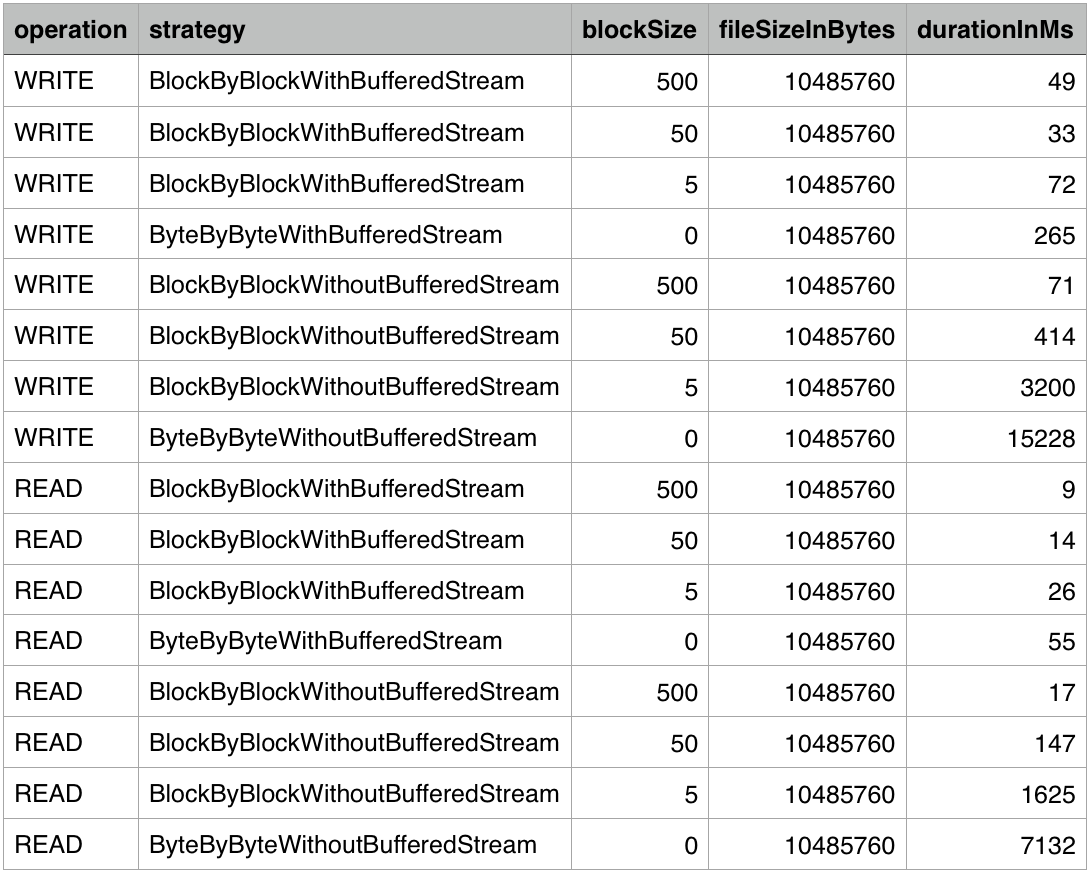
\includegraphics[width=400pt]{images/results.png}
		
		\pagebreak
				
		\justify
		
		\subsection{Comparaison des vitesses de lecture et d'écriture}
			\noindent 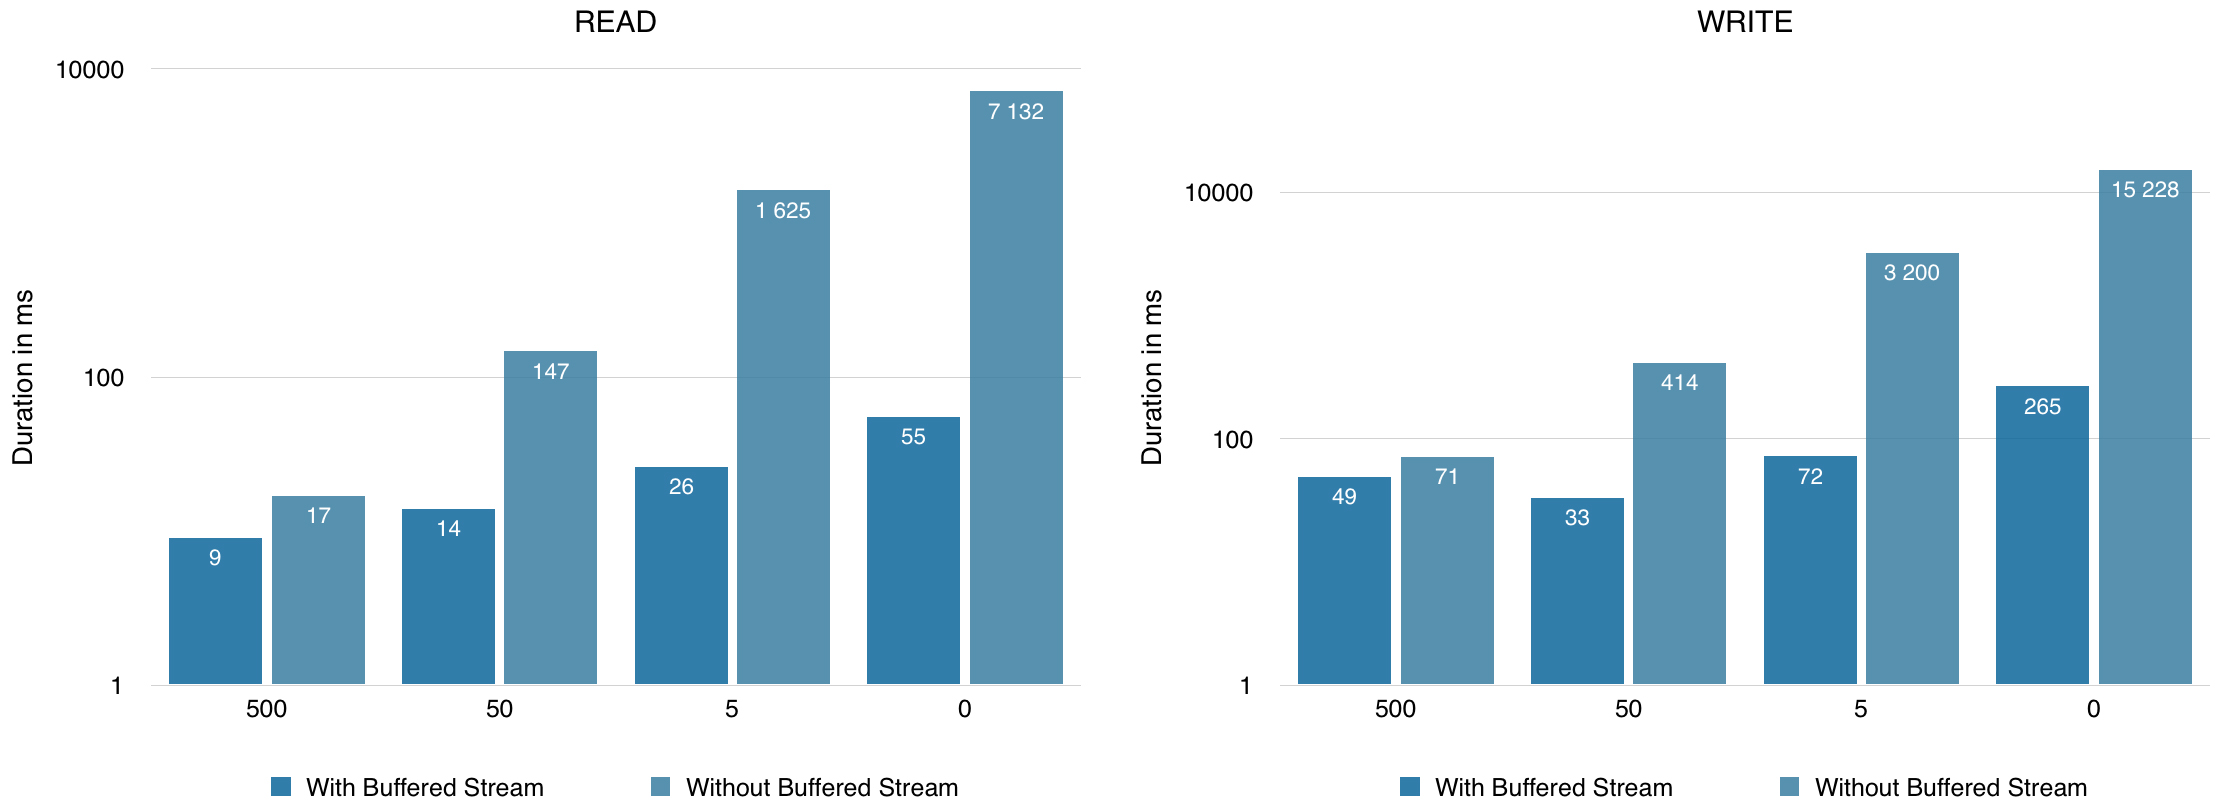
\includegraphics[width=480pt]{images/graphiques.jpg} \\
			
			\noindent L'utilisation du buffer apporte un gain de vitesse conséquent lors de la lecture, notamment lors de la lecture de petits blocs voir même de simples Bytes. Ceci, car comme vu durant le cours, les buffers permettent de "pré-charger" plusieurs Bytes (en fonction de la taille du buffer) même lors de la lecture d'un seul Byte. Ainsi, si une nouvelle lecture doit être faite, celle-ci sera effectuée en mémoire et non dans le fichier directement (ou un autre support), ce qui est beaucoup plus rapide. C'est pour ça que plus les blocs lus sont petits, plus il est nécessaire de retourner lire le fichier. \\
			
			\noindent Il en est de même pour l'écriture dans un fichier. Plus les blocs sont petits, plus le temps de lecture total est grand.
				
	\section{Modification du programme}
		\noindent Afin d'enregistrer les résultats dans un fichier CSV, les classes ont été implémentées comme expliqué dans l'exemple mis à notre disposition. \\
		
		\noindent Un point particulier à relever concerne la classe \textbf{BenchmarkExperimentData} destinée à contenir toutes les informations d'un test. Ces données sont stockée sous forme d'attributs (String et Long) qui sont ensuite transmis à l'aide d'une liste à l'objet CsvSerializer. Celui-ci n'a ensuite plus qu'à traiter chaque élément à la suite afin de créer une chaîne une chaine de caractères dans l'ordre souhaité à destination du fichier CSV. \\
		
		\noindent Dans le programme principal, le \textbf{recorder} est un attribut static qui va récolter les données des tests au fûr et à mesure qu'ils sont effectués. L'initialisation de cet objet se fait directement dans la méthode main. Il lui est transmis le chemin vers le fichier de sortie, ainsi que le serializer à utiliser (ici CsvSerializer). Un premier record est ensuite enregistré sous forme d'un objet IData anonyme qui va simplement redéfinir la méthode getValues() pour retourner les en-têtes du fichier CSV. En fin de programme, le recorder est fermé ce qui entraine, dans le cas d'un FileRecorder, la fermeture du fichier. \\
		
		\noindent Le resultat des tests est transmis en deux endroits au recorder : à la fin des méthodes produceTestData() et consumeTestData(). Ceci est fait en créer une nouvelle instance de BenchmarkExperimentData contenant les données souhaitées et en transmettant cet objet au recorder au travers de la méthode record(). \\
		\noindent La méthode consumeDataFromStream() a également été modifiée afin de retourner le nombre de Bytes lus, pour que ce dernier soit inclus dans le fichier CSV.
	
\end{document}
